
\documentclass[12pt]{article}
\usepackage[spanish]{babel}
\usepackage{booktabs}
\usepackage{longtable}
\usepackage{latexsym}
\usepackage{lipsum}
\usepackage{graphicx}
\usepackage{tikz}


\textwidth     =  6.5in
\textheight    =  9.0in
\oddsidemargin =  0.2in
\topmargin     = -0.6in
\usepackage{amsmath, amssymb, latexsym}


%%%%%%%%%%%%%%%%%%%%%%%%%%%%%%%%%%%%%%%%%%%%%%%%%%%%%%%%%%%%%%%%%%%%%%%%
\newcommand{\be}{\begin{equation}}
\newcommand{\ee}{\end{equation}}
\newcommand{\bes}{\begin{equation*}}
\newcommand{\ees}{\end{equation*}}

\newcommand{\bea}{\begin{eqnarray}}
\newcommand{\eea}{\end{eqnarray}}

\newcommand{\beas}{\begin{eqnarray*}}
\newcommand{\eeas}{\end{eqnarray*}}

\newcommand{\bet}{\begin{tabular}}
\newcommand{\ent}{\end{tabular}}
\newcommand{\mul}{\multicolumn}
\newcommand{\bec}{\begin{center}}
\newcommand{\enc}{\end{center}}
\newcommand{\bei}{\begin{itemize}}
\newcommand{\eni}{\end{itemize}}
\newcommand{\bee}{\begin{enumerate}}
\newcommand{\ene}{\end{enumerate}}
\newcommand{\noi}{\noindent}
\newcommand{\unl}{\underline}
\newcommand{\ul}{\underline}
\newcommand{\real}{\mathbb{R}}
\newcommand{\feal}{\mathbb{F}}
\newcommand{\natu}{\mathbb{N}}
\newcommand{\fact}{\mathbb{X}}

\def\checkmark{\tikz\fill[scale=0.4](0,.35) -- (.25,0) -- (1,.7) -- (.25,.15) -- cycle;} 

\begin{document}
\title{TDA: Proyecto final}
\author{Guillermo Santiago Novoa P\'erez\\  \small{125089}
}
\date{ 18 de mayo de 2016.}
\maketitle
\noi En este trabajo se utilizaron t\'ecnicas de an\'alisis topol\'ogico para intentar encontrar relaciones no lineales en nuestra base de datos. \\ \\ \\
{\underline{\large{Base de datos: d\'igitos }}}\\ \\
\noi Esta base de datos se encuentra en la libreria 'ElemStatLearn' de r y puede ser llamada con 'data(zip.train)', es muy conocida ya que ofrece un buen ejemplo para diferentes problemas de clasificaci\'on y reducci\'on de dimensionalidad. La base de datos trae un total de 7291 n\'umeros del 0 al 9 escritos a mano, parametrizados por 258 cuadr\'iculas ( o variables ).  En particular, este ejemplo se usa en el reconocimiento de d\'igitos escritos a mano.\\
\indent El problema ha capturado la atenci\'on de la comunidad de aprendizaje de m\'aquina por muchos a\~{n}os y sigue siendo un problema de referencia para cualquier cient\'ifico de datos.\\ \\ \\
{\underline{\large{Algoritmo}}}\\ \\
\noi Nuestro algoritmo de clasificaci\'on tiene las siguientes alternativas para hacer la gr\'afica final:
\bei
\item Elecci\'on del filtro
\bei
\item Cualquiera de las 258 variables originales.
\item El primer eigenvector de los datos transformados con el algoritmo de Laplacian Eigenmaps (LE).
\item Crear un grid con los dos primeros eigenvectores de los datos transformados con LE.\footnote{El algoritmo de Laplacian Eigenmaps a su vez tiene la opci\'on de elegir los pesos de las distancias entre puntos con un enfoque sencillo (ceros y unos) o usando el "heat kernel"\ como medida de distancia. Para encontrar qu\'e puntos estaban conectados se utiliz\'o k-vecinos m\'as cercanos.}
\eni
\item Clustering
\bei
\item El clustering se hace con el algoritmo de BFS.
\eni
\eni 
\pagebreak
{\underline{\large{Implementaci\'on}}}\\ \\
\noi Se implement\'o nuestro algoritmo utilizando como filtro los dos primeros valores propios del algoritmo de Laplacian Eigenmaps, para los pesos se us\'o el heat kernel.\\
\indent Los par\'ametros utilizados fueron los siguientes:
\bei
\item Filtro (LE)
\bei
\item $n = 5$\ \ \           {\it{n\'umero de vecinos m\'as cercanos}}
\item $t = 10$\ \ \          {\it{par\'ametro del kernel del calor}}
\eni
\item Intervalos
\bei
\item $n_{int1} = 3$\ \ \       {\it{n\'umero de intervalos en los que se va a separar el primer eigenvalor de LE}}
\item $n_{int2} = 2$\ \ \       {\it{n\'umero de intervalos en los que se va a separar el segundo eigenvalor de LE}}
\eni
\item Clustering
\bei
\item $n_2 = 5$\ \ \          {\it{n\'umero de vecinos que se utilizar\'an para checar el \'arbol }}     
\eni
\eni
$$$$
\noi Primero veamos c\'omo quedan nuestros datos graficados en los dos filtros que estamos usando para pensar qu\'e nos deber\'ia quedar en el resultado y si hace alg\'un sentido. 
$$$$
\begin{figure}[h!]
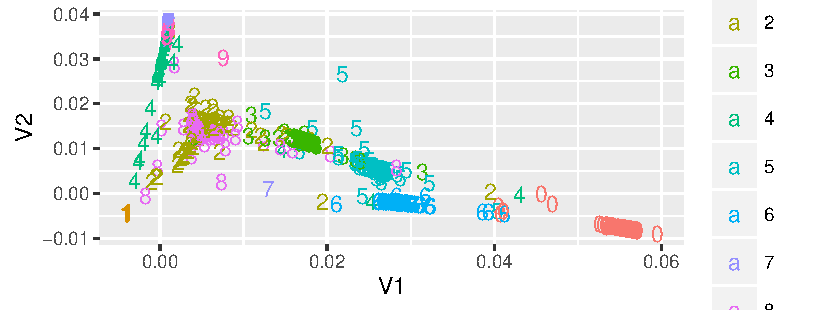
\includegraphics[trim={5cm .5cm 5cm .5cm},width=0.25\textwidth]{digits_good.pdf}
\centering
\end{figure}
\noi Si nuestro algoritmo funcionara podr\'iamos ver ciertas relaciones entre varios n\'umeros, seises y cincos, treses y cincos, ochos y doses, y hasta unos y cuatros; adem\'as, s\'olo fij\'andonos en la primer componente (primer eigenvector del LE), los ceros y los unos toman papeles opuestos.\\
\pagebreak

{\underline{\large{Resultados}}}\\
\begin{figure}[h!]
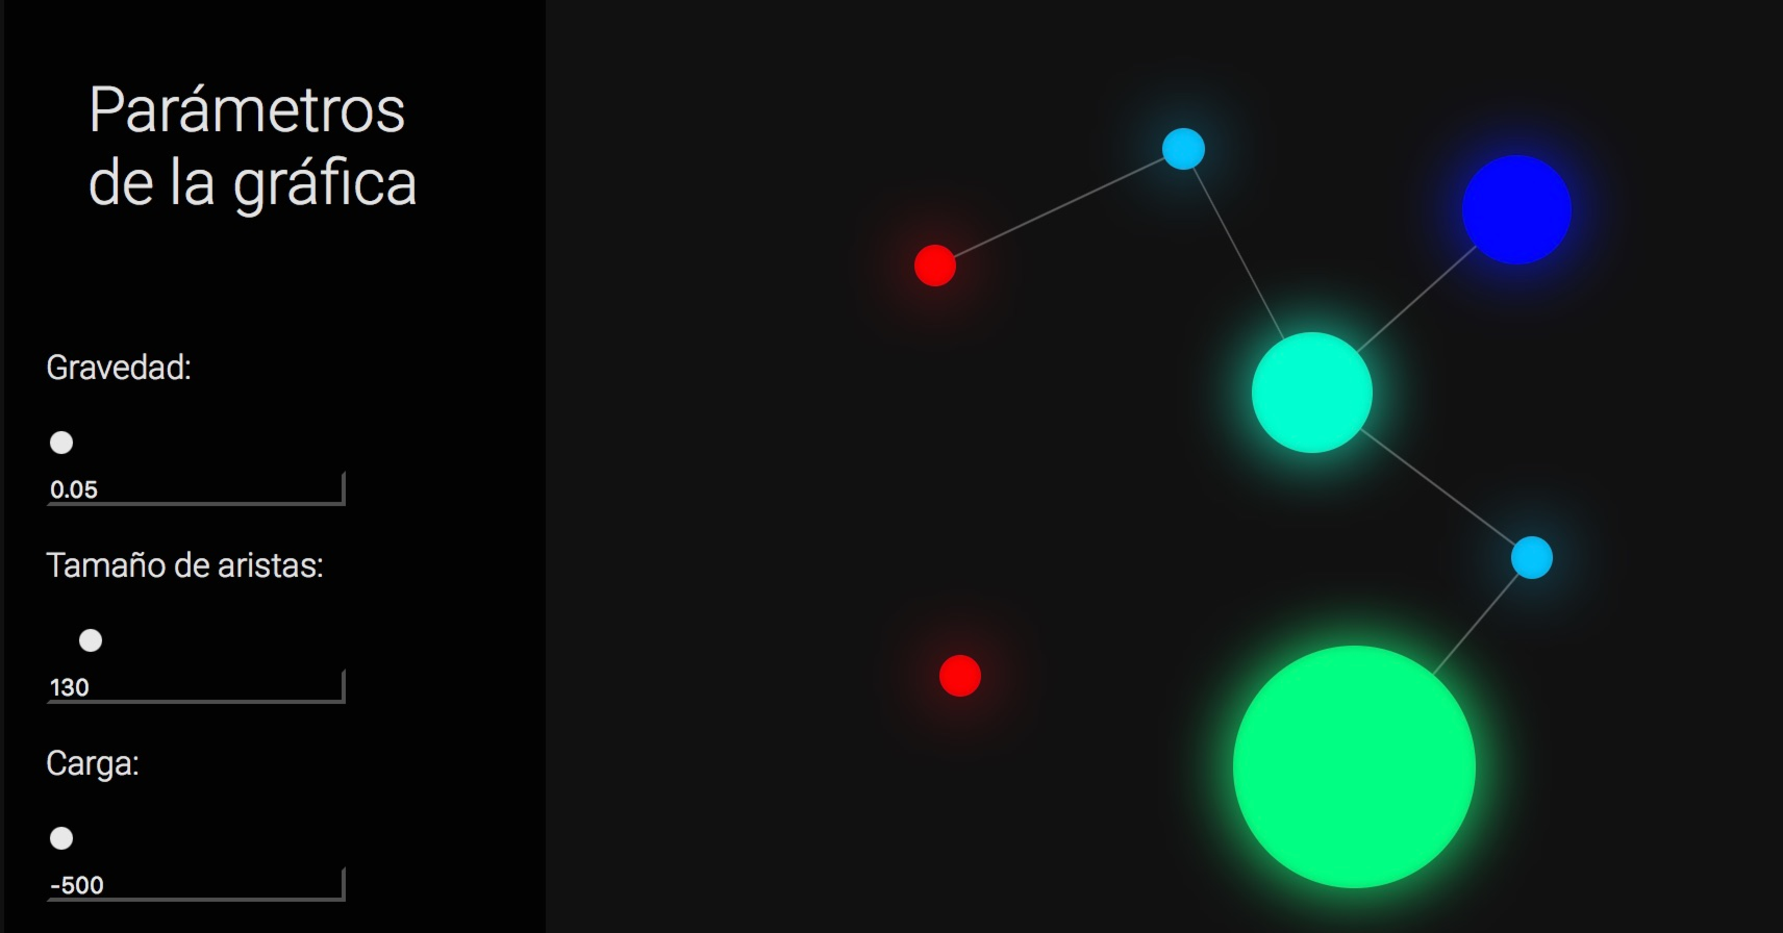
\includegraphics[trim={5cm .5cm 5cm .5cm},width=0.45\textwidth]{graf_iso}
\centering
\end{figure}
\begin{figure}[h!]
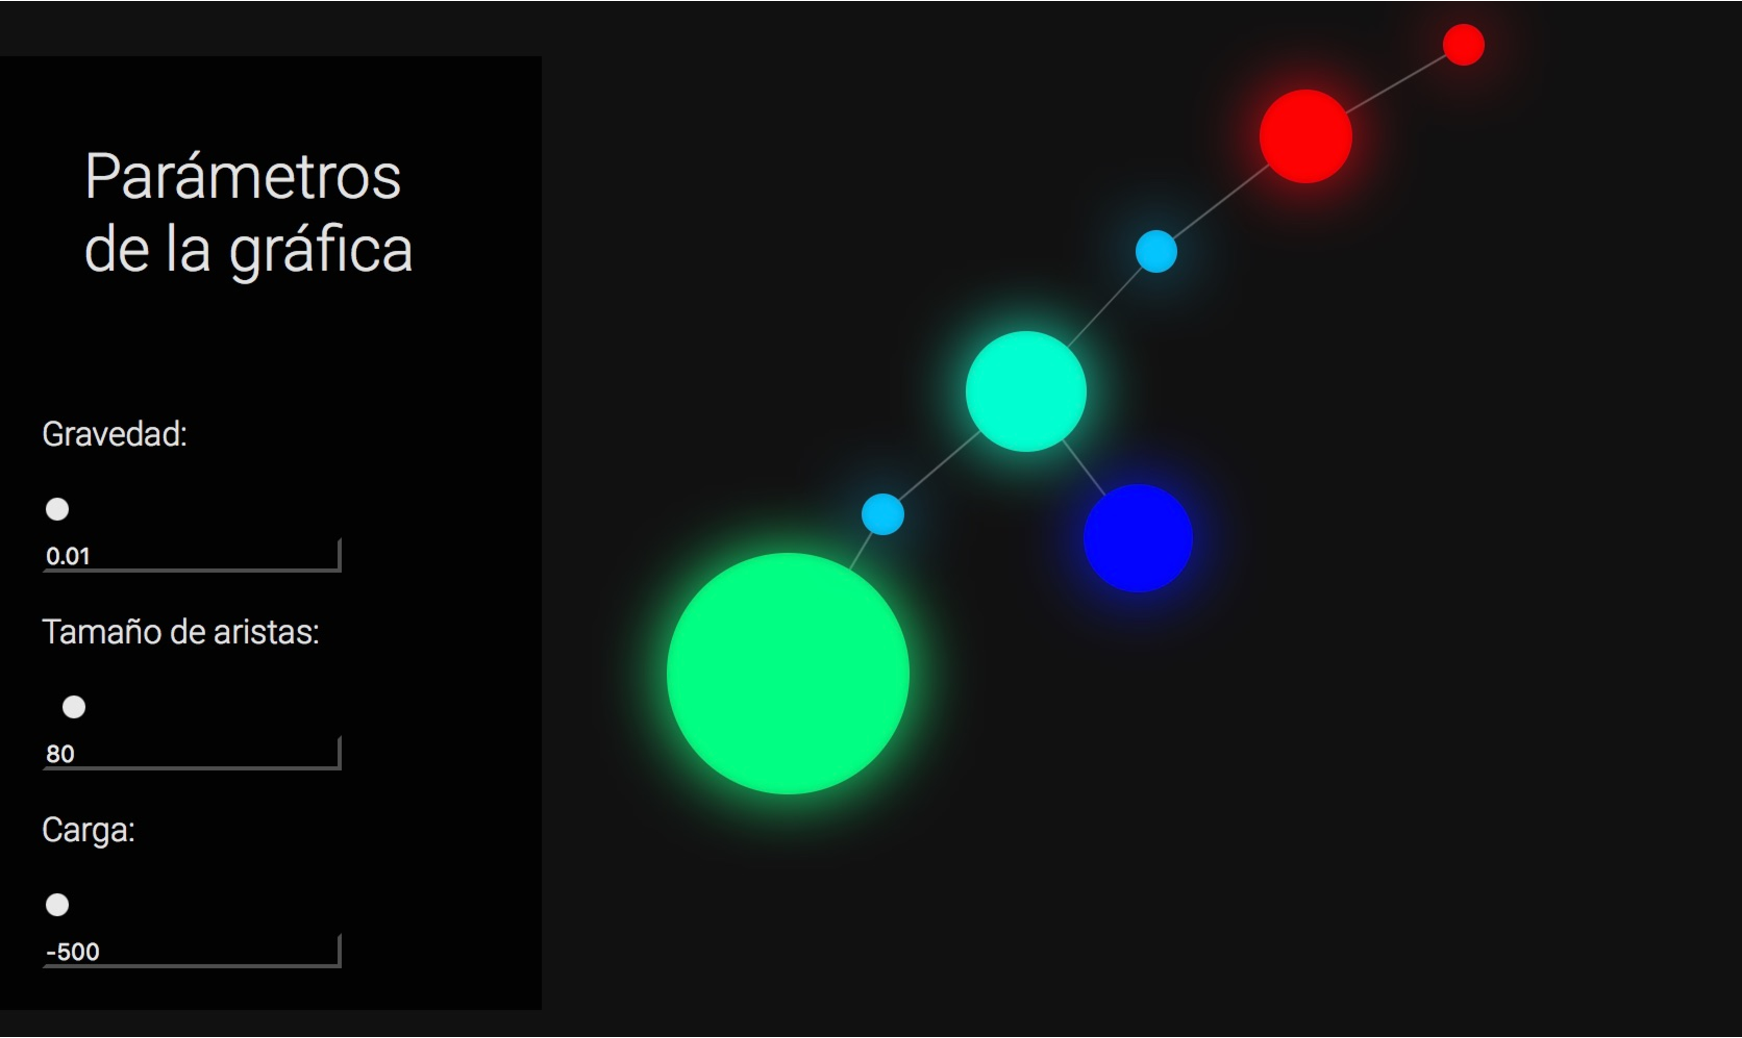
\includegraphics[trim={5cm .5cm 5cm .5cm},width=0.45\textwidth]{graf_uni}
\centering
\end{figure}\\
\noi En las dos gr\'aficas existe un nodo que se aleja de los dem\'as, en este nodo se encuentran todos los 0's (en una de las gr\'aficas es una isla, en otra est\'a al extremo). Contrario a este nodo siempre se encuentran aglomerados los 1's (que est\'an cercanos a los 2's). Los nodos del centro contienen a los 5's y 6's, adem\'as de los 3's en mucho menor escala.\\
\indent En si podemos decir que para valores en la izquierda del primer eigenvector se encuentran la mayor\'ia de los n\'umeros ya que el tama\~{n}o de la primer bola es mucho mayor a las dem\'as (1's, 4's, 9's, 7's, 8's y 2's), y conforme se va yendo a la derecha nacen otros grupos (que contienen curvas o loops) terminando con el cero siendo el m\'as "redondo". La segunda componente principal (o el segundo eigenvalor del algoritmo LE) no aparece para valores cercanos al cero (parece que s\'olo divide a n\'umeros que no son redondos) y puede hablar del n\'umero de cortes que tiene cada n\'umero, por ejemplo, los 5's tienen valores altos y bajos de esa componente, mientras que los 7's y los 4's son los que mayores valores alcanzan.\\
\indent Viendo s\'olo nuestras dos gr\'aficas finales, lo que m\'as sobresale es la diferencia entre unos (palos) y ceros (bolas), pasando por todos los n\'umeros en medio que parecen clasificarse por dos cosas, n\'umero de cortes (por eso la separaci\'on entre los cincos y seises) y redondez del n\'umero. 
\end{document}  